\documentclass[aspectratio=169]{beamer}

% Configuración básica del tema
\usepackage{lmodern} % Fuente moderna
\usepackage[utf8]{inputenc} % Soporte para caracteres UTF-8
\usepackage[spanish]{babel} % Idioma español
\usepackage{amsmath} % Matemáticas avanzadas
\usepackage{minted}
\usepackage{listings}
\usepackage{xcolor}

% Tema minimalista
\usetheme{default}

% Definir colores
\definecolor{customblue}{RGB}{45, 85, 150}

% Personalización del encabezado
\setbeamercolor{frametitle}{bg=customblue, fg=white}
\setbeamercolor{section in head/foot}{fg=customblue}

% Configuración del diseño
\setbeamertemplate{frametitle}{
    \nointerlineskip%
    \begin{beamercolorbox}[wd=\paperwidth, ht=2.5ex, dp=1.5ex]{frametitle}
        \usebeamerfont{frametitle}\hspace{1em}\insertframetitle
    \end{beamercolorbox}
    \vspace{0.5em}
    \nointerlineskip%
    \rule{\paperwidth}{0.2mm}
}

\setbeamertemplate{footline}[frame number]

\lstdefinestyle{mystyle}{
    backgroundcolor=\color{gray!10},
    basicstyle=\ttfamily\small,  % Fuente monoespaciada
    breaklines=true,
    frame=single,
    keywordstyle=\color{blue},
    commentstyle=\color{gray},
    stringstyle=\color{red},
    columns=fullflexible  % Evita problemas de espaciado
}
\lstset{style=mystyle}

% Inicio del documento
\begin{document}

% Primera diapositiva: Título
\begin{frame}
    \centering
    \vspace{1.5cm}
    \Huge \textbf{Chuletario Ejercicios Tema 1} \\
    \Large Lo que Dijkstra, Anna Karlin y Donald Knuth no quieren que sepas
    \vfill
    \normalsize \textit{Metodología de la Programación} \\
    \small \textbf{Autor: Víctor Alonso} % Modifica tu nombre si lo deseas
\end{frame}

% Ejemplo de diapositiva con contenido
\section{Orden de Complejidad}

\begin{frame}{Orden de Complejidad}
    \begin{itemize}
        \item \textbf{¿Qué es?:} Estudiar el \textbf{comportamiento} de un algoritmo.
        \item \textbf{Pasos:}
        \begin{enumerate}
            \item Identificar \textbf{condición de salida} del bucle.
            \item Estimar el número de iteraciones con \textit{tablita} o fórmula.
            
            \item Plantear T(n).
        \end{enumerate}
        \item \textbf{Bro tips:} 
       \begin{itemize}
            \item Un número \textit{fijo} de iteraciones no tiene impacto en el orden.
            \item Nos da igual \textit{n} iteraciones que \textit{n-m} iteraciones.
            \[
                \forall m \in \mathbb{Z}
            \]
        \end{itemize}
    \end{itemize}
\end{frame}

\begin{frame}{Orden de Complejidad (notación matemática)}
    \begin{itemize}
        \item \textbf{T(n)}: Función de complejidad. Planteamos el problema con operaciones definidas (a, b, c...), y sumatorios para los bucles.
        \[
            T(n) = a + \sum_{i=0}^n b
        \]
        \item \textbf{Orden de complejidad equivalente:} Usamos la \textit{virgulilla} encima del \textit{igual} para decir que las expresiones son \textbf{equivalentes en cuanto a orden de complejidad}.
        \[
        T(n) = a + \sum_{i=0}^n b \overset{\sim}{=} a + bn
        \]
        \item \textbf{Polinomios}: Nos quedamos con el término \textbf{n} elevado al mayor exponente. Y ese será el O(n).
        \[
            T(n) = a + \sum_{i=0}^n b \overset{\sim}{=} a + bn
            \]
            \[
            T(n) \in \mathcal{O}(n), \ \Omega(n) \ \Rightarrow \ T(n) \in \Theta(n)
        \]
    \end{itemize}
\end{frame}

\begin{frame}{Orden de Complejidad (Bro tips)}
\textbf{¿Por qué descartamos todo lo que no sea \textit{n elevado al mayor exponente}?}
    \begin{itemize}
        \item Las funciones \textbf{se comportan igual} independientemente de los \textit{términos sueltos}.
        \item Solo nos interesa saber cómo crece. No buscamos rapidez en \textit{términos absolutos}, sino \textit{comportamientos} \textbf{eficientes}.
    \end{itemize}

    % Insertar la imagen
\begin{figure}[h!]
    \centering
    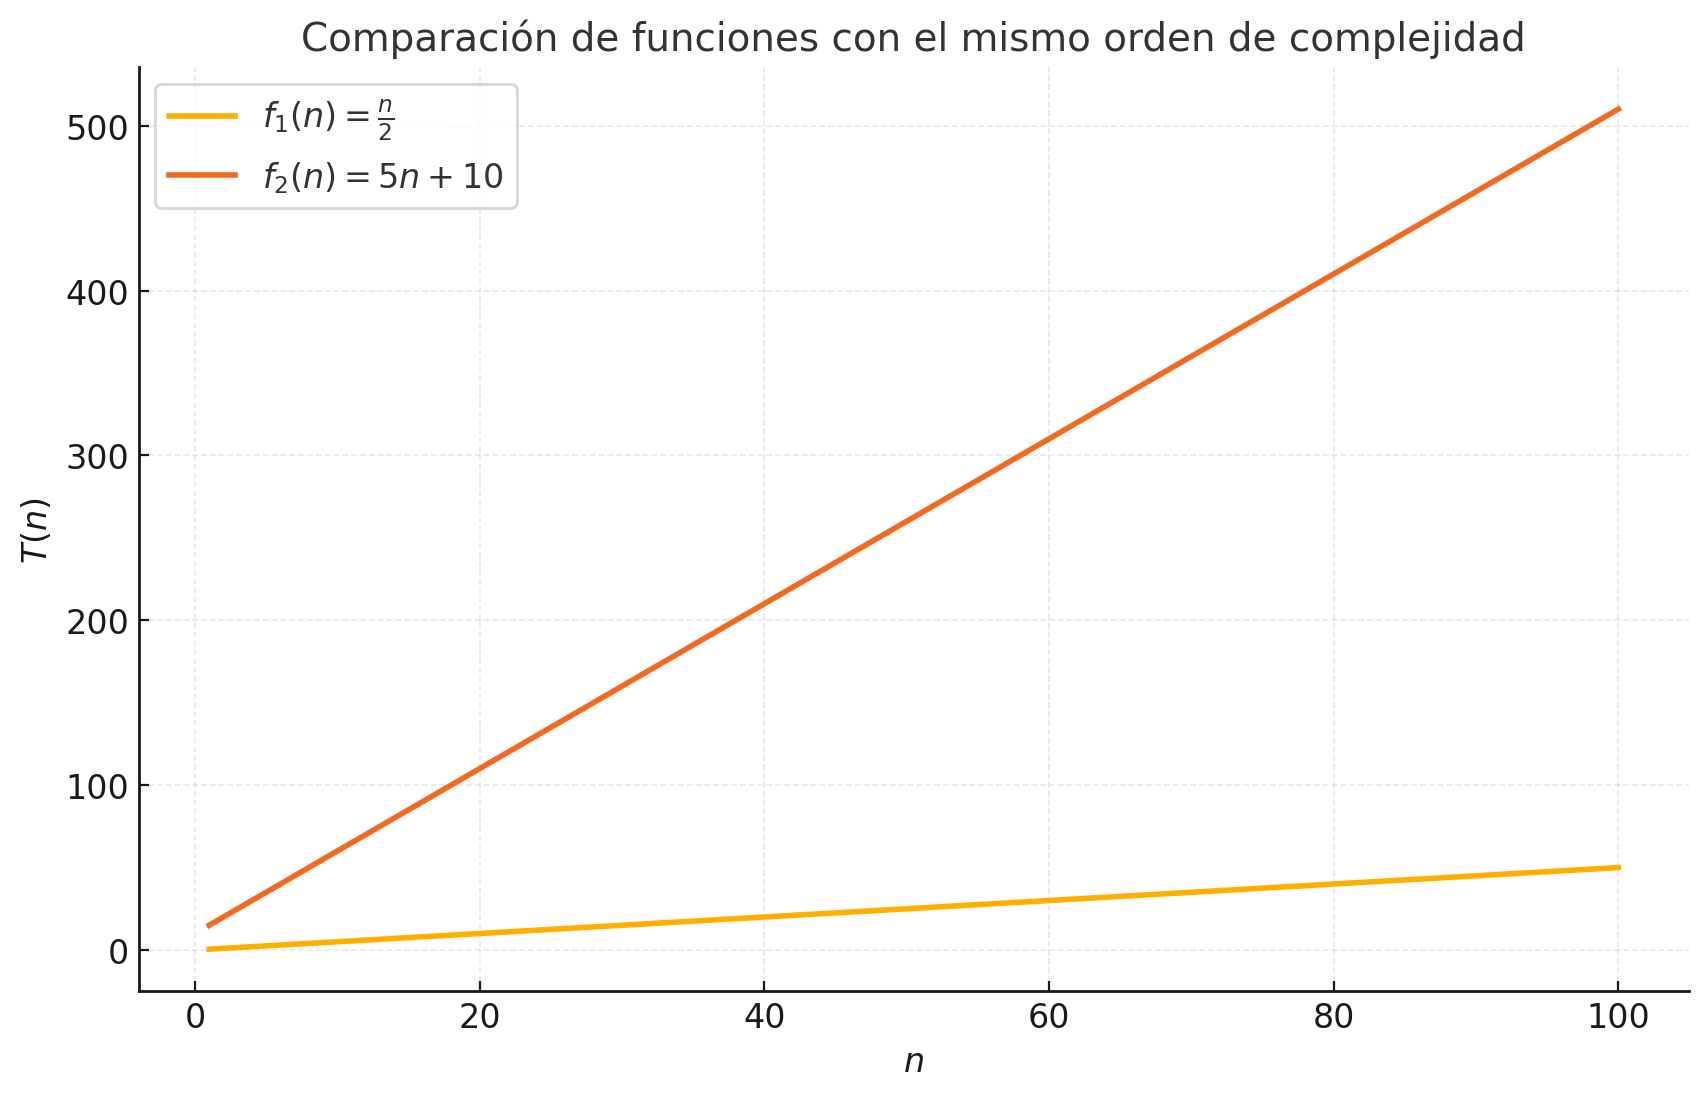
\includegraphics[width=0.5\textwidth]{orden-n.png}
    \caption{Gráfica que muestra que \(f_1(n)\) y \(f_2(n)\) tienen el mismo orden de complejidad.}
    \label{fig:orden-n}
\end{figure}
\end{frame}

\begin{frame}{Orden de Complejidad (Bro tips 2)}
\textbf{¿Por qué tienen el mismo orden de complejidad las funciones de la gráfica?}
\begin{itemize}
    \item La derivada de \(f_1(n) = \frac{n}{2}\) es \(f_1'(n) = \frac{1}{2}\), y la derivada de \(f_2(n) = 5n + 10\) es \(f_2'(n) = 5\). Ambas son constantes, lo que indica \textbf{crecimiento lineal}.
    \item Aunque \(f_2(n)\) crece más rápido que \(f_1(n)\), ambas funciones tienen el mismo tipo de crecimiento: \textbf{proporcional a \(n\)}.
    \item En términos de complejidad, \textbf{solo importa el comportamiento asintótico} para \(n\) grande, por lo que las constantes y términos independientes son irrelevantes.
    \item Esto demuestra que ambas funciones están en el mismo orden de complejidad, \(\mathcal{O}(n)\). Aunque los algoritmos \textbf{no tarden el mismo tiempo exacto}.
    \item El crecimiento de estas funciones es continuo y uniforme, a diferencia de otros tipos de crecimiento (e.g., \(n^2\) o \(\log n\)).
\end{itemize}

\end{frame}

% Nueva sección (puedes copiar y pegar este formato para añadir más diapositivas)
\section{Análisis de un bucle}

\begin{frame}[fragile]{Número de iteraciones}
\begin{verbatim}
j = n
k = 1
while j >= 1
    k = k + 1
    j = n / k
\end{verbatim}

\begin{itemize}
    \item \textbf{Buscamos condición de salida:} El bucle termina cuando \(j < 1\). Pero podemos \textit{aproximarlo} a \(j = 1\).
    \item \textbf{¿Cuándo se cumple?:} Analizamos las operaciones en \(j\):
    \begin{itemize}
        \item \(j = n / k\), por lo que \(j = 1\) cuando \(n / k = 1\), es decir, cuando \(k = n\).
        \item Como \(k\) aumenta de uno en uno (\(k = k + 1\) en cada iteración), el bucle ejecutará \(n\) iteraciones.
    \end{itemize}
    \item \textbf{Bro Tip}: A veces no hace falta \textit{tablita mágica}.
\end{itemize}
\end{frame}


\begin{frame}{Cosas que quedan bien}
\textbf{Índices del sumatorio}

\begin{itemize}
    \item Es importante fijarse en \textbf{dónde empieza el bucle} para definir correctamente el índice inferior del sumatorio.
    \item En el caso anterior:
    \[
    \sum_{k=1}^n
    \]
    El bucle empieza en \(k = 1\) y termina en \(k = n\).

    \item Sin embargo, en otros casos, el bucle puede \textit{ir al revés}. Por ejemplo el ejercicio 4. Si lo expresamos en términos de un sumatorio:
    \[
    \sum_{i=\log_5 n}^1
    \]

    \item \textbf{Bro tip:} Da igual cómo se pongan los límites del sumatorio porque representan las mismas iteraciones. Lo importante es reflejar correctamente el comportamiento del bucle.
\end{itemize}

\end{frame}

\section{Bucle anidado}

\begin{frame}{Bucle anidado y sumatorios}
\[
T(n) = a + \sum_{i=0}^n \left( b + \sum_{k=0}^n c \right)
\]

\begin{itemize}
    \item El primer sumatorio (\(\sum_{i=0}^n\)) representa el bucle exterior, el segundo sumatorio (\(\sum_{k=0}^n\)) representa el bucle interior.
    \item Resolvemos primero el sumatorio del bucle interior:
    \[
        T(n) = a + \sum_{i=0}^n \left( b + cn \right)
    \]
    \item Resolvemos después del otro sumatorio.
    \[
        T(n) = a + bn + cn^2
    \]
   \end{itemize}

   \[
T(n) = a + \sum_{i=0}^n \left( b + \sum_{k=0}^n c \right) \overset{\sim}{=} a + \sum_{i=0}^n \left( b + cn \right) \overset{\sim}{=} a + bn + cn^2
\]
\end{frame}


\begin{frame}{Bro Tips para resolver sumatorios}
\begin{itemize}
    \item \textbf{Poner \(a\), \(b\), \(c\)...:} Identifica claramente las constantes y dónde aparecen en el bucle.
    \item \textbf{Poner paréntesis:} Agrupa las operaciones correctamente para no perder términos en cada paso.
    \item \textbf{\(b\) son las operaciones antes del bucle:} Estas se SUMAN a las del sumatorio interior, y deben incluirse fuera del segundo sumatorio.
    \item \textbf{Resolver paso a paso:} Simplifica un sumatorio a la vez para evitar errores y asegurar que el resultado final sea correcto.
\end{itemize}
\end{frame}

\begin{frame}{Ultimate BRO TIP: Bucles anidados 1 }
\begin{figure}
    \centering
    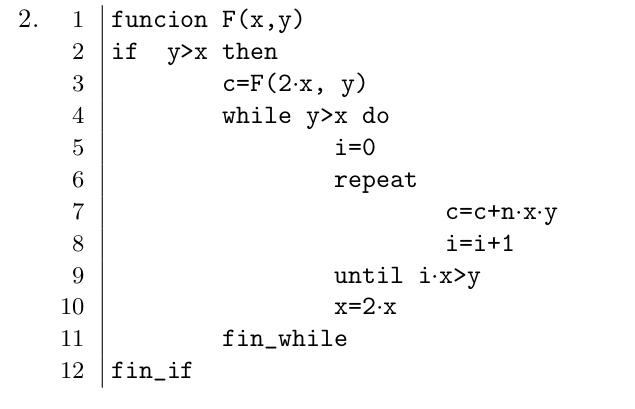
\includegraphics[width=0.5\linewidth]{sumatorio-ejercicio.png}
    \label{fig:enter-label}
\end{figure}
\textbf{Explicación:} 
En este código, el bucle exterior se ejecuta mientras $y > x$, y en cada iteración, $x$ se duplica. Esto lleva a un número total de iteraciones de $O(\log n)$. Por otro lado, el bucle interno se ejecuta un número de veces dependiente de $x$, por lo que despejamos su número de vueltas en función de las vueltas del exterior.
\end{frame}

\begin{frame}{Ultimate BRO TIP: Bucles anidados 2}
\begin{itemize}
    \item \textbf{Identificar iteraciones y tamaño del problema:} 
    Nuestro tamaño del problema es una variable que tomaremos para simplificar los cálculos. En este caso la llamaremos \textit{m}. \(m = y/x\). El bucle exterior se ejecuta $\log_2 m$ veces, lo que denominamos $j$.
    
    \item \textbf{Determinar el bucle interior:} 
    En cada iteración del bucle exterior, el número de iteraciones del interior \textbf{depende del valor actualizado de la variable $x$}, o de nuestra nueva variable m. 
    Para cada $j$, el bucle interior ejecuta $2^j$ iteraciones (despejamos la m en la fórmula del bucle exterior).
    \[ j = log_2 m  => m = 2^j \]

    \item Tomemos \(y = 32\) y \(x = 1\). El bucle exterior se ejecuta \(log_232 = 5\) veces.
    \item El interior se ejecuta: 17 veces, luego 9, 5 veces, ...
    \item En realidad es \(2^j + 1\) veces, pero sabemos que una iteración no afecta al orden de complejidad.
\end{itemize}
\end{frame}

\begin{frame}{Ultimate BRO TIP: bucles anidados 3}
\begin{itemize}

    \item \textbf{Plantear el sumatorio:} 
    La cantidad total de iteraciones es:
    \[
        \sum_{j=0}^{\log_2 m} 2^j
    \]
    Resolviendo el sumatorio:
    \[
        \sum_{j=0}^{\log_2 m} 2^j = 2^{\log_2 m* } = 2m  \approx O(m)
    \]
    
    \item \textbf{Conclusión:} 
    A pesar de tener un bucle exterior de $O(\log m)$, el total de iteraciones es $O(m)$ debido al impacto del bucle interior.
    \item *Recuerda que \(a^{log_ab} = b\)
\end{itemize}
\end{frame}

\begin{frame}{Función de recurrencia}
Identificar la recurrencia:
\begin{itemize}
    
    \item \textbf{Ver las veces que se llama:} Analizar si la función se llama a sí misma y cuántas veces en cada iteración. Además, tiene que llamarse con algún cambio cada vez (si no sería un bucle infinito), es \textbf{importante identificar qué cambia}.
    
    \item \textbf{Ojo al manojo:} Si hay un número multiplicando la llamada recursiva, suele ser un multiplicador del resultado final, pero no necesariamente el número de llamadas. \textbf{It's a trap!}
    
    \item \textbf{Buscar si está en un bucle:} Interpretar el número de llamadas REALES considerando la interacción con estructuras de control como bucles.
\end{itemize}
\end{frame}


\begin{frame}[fragile]{Trampas para aventureros incautos}
\textbf{Ejemplo 1: Llamadas en un bucle}
\begin{lstlisting}
function Q(a, b)
    for i = 1 to 3 do
        Q(a/2, b)
    end for
end
\end{lstlisting}
\textbf{Explicación:} 
En cada iteración del bucle, la función se llama con $a/2$. Como el bucle se ejecuta 3 veces, se hacen exactamente 3 llamadas recursivas.

\textbf{Ejemplo 2: Multiplicador en la llamada}
\begin{lstlisting}
z = 3 * Q(1,2)
\end{lstlisting}
\textbf{Explicación:} 
Aquí, $Q(1,2)$ se llama solo una vez. El 3 no significa que haya 3 llamadas, sino que su resultado se multiplica por 3.
\end{frame}

\begin{frame}{Función de recurrencia (análisis detallado)}
\begin{itemize}
    \item \textbf{Identificar las llamadas recurrentes y con qué valores:} 
    Analizar cómo cambian los parámetros en cada llamada. Esta parte es conocida como la \textbf{parte homogénea} de la recurrencia.
    
    \item \textbf{Poner el resto de costes no recurrentes:} 
    Identificar operaciones externas a la recurrencia, que constituyen la \textbf{parte no homogénea o particular}.
\end{itemize}

\textbf{Ejemplo:}
\[
T(n) = 3T(n-1) - 8T(n-2) + 4T(n-3) + n^2 - 1
\]
\begin{itemize}
    \item La \textbf{parte homogénea} es \( 3T(n-1) - 8T(n-2) + 4T(n-3) \), ya que describe las llamadas recursivas y cómo cambian los parámetros.
    \item La \textbf{parte no homogénea} es \( n^2 - 1 \), que representa el coste adicional fuera de la recursión.
\end{itemize}
\end{frame}

\begin{frame}{Ecuación característica 1}
\begin{itemize}
    \item Buscamos la \textbf{ecuación característica}.
    \item \textbf{Para la parte homogénea} suponemos una solución de la forma \( T(n) = r^n \) y sustituimos en la ecuación homogénea (donde pone T(n) ponemos \( r^n\)):
    \[
    r^n = 3r^{n-1} - 8r^{n-2} + 4r^{n-3}
    \]
    \item Dividimos por \( r^{n-3} \) (\textbf{el menor exponente presente}) para obtener una ecuación polinómica:
    \[
    r^3 - 3r^2 + 8r - 4 = 0
    \]
    \item Resolvemos buscando las raíces del polinomio, generalmente con Ruffini o factorización directa (para grados 3 o más) o con la ecuación de segundo grado si es cuadrática.
\end{itemize}
\end{frame}

\begin{frame}{Ecuación característica 2}
\begin{itemize}
    \item Cada solución de la ecuación homogénea se expresa en la forma \( (x - \text{raíz}) \).
    \item Se factorizan todas las raíces encontradas para obtener la forma factorizada del polinomio.
    \item Una vez obtenida la forma factorizada, guardamos estas soluciones y nos dirigimos a analizar la parte no homogénea.
\end{itemize}
\end{frame}

\begin{frame}{Parte no homogénea polinómica}
\begin{itemize}
    \item Buscamos el término de mayor grado en la parte no homogénea.
    \item Si el término de mayor grado es \( n^k \), generamos \( (x - 1)^{k+1} \).
    \item Esto asegura que la forma de la solución particular tenga en cuenta la estructura del término no homogéneo.
\end{itemize}

\textbf{Ejemplo:}
\[
T(n) = 3T(n-1) - 8T(n-2) + 4T(n-3) + n^2 - 1
\]
\begin{itemize}
    \item El término de mayor grado en la parte no homogénea es \( n^2 \), por lo que generamos \( (x - 1)^3 \).
\end{itemize}
\end{frame}

\begin{frame}{Parte no homogénea exponencial}
\begin{itemize}
    \item Si la parte no homogénea es de la forma \( (n^k * P(n))r^n \), generamos \( (x - r)^{k+1} \).
    \item Esto garantiza que la solución particular refleje la estructura exponencial.
\end{itemize}

\textbf{Ejemplo:}
\[
T(n) = 2T(n-1) - 5T(n-2) + (n-5)3^n
\]
\begin{itemize}
    \item La parte no homogénea es \( (n-5)3^n \), por lo que generamos \( (x - 3)^2 \). O sea, x menos la base elevado al mayor exponente del polinomio + 1.
\end{itemize}
\end{frame}


\begin{frame}{Ecuación característica 3}
\begin{itemize}
    \item Una vez obtenidas las raíces la ecuación característica se expresa como:
    \[
    (x-r_1)*(x-r_2)^k = 0 
    \]
    donde \( r_1, r_2 \) son las raíces que hemos sacado. Si tiene más raíces se ponen, claro.
    
    \item {Ejemplo:} Si la ecuación característica es \( (x-2)(x-3)^2 = 0 \), las raíces son \( r_1 = 2 \) y \( r_2 = 3 \) con multiplicidad 2. La solución general es:
        \[
        T(n) = C_1 2^n + (C_2 + C_3n) 3^n
        \]
    \item Para encontrar los coeficientes \( C_1, C_2, C_3 \), se usan las condiciones iniciales de la recurrencia.
\end{itemize}
\end{frame}


\begin{frame}{Ecuación característica Bro tips}
\begin{itemize}
    \item Tendremos constantes \( C_1, C_2, C_3, C_4, ... \) multiplicando a \textbf{la raíz simple} que esté elevada a n.
    \item Para las múltiples tendremos tantas constantes nuevas como el exponente de la raíz, empezando por grado 0 hasta grado \textit{exponente - 1}. Y todo eso multiplicando a la raíz múltiple elevada a n. Observa como \[ (x-3)^2\] pasa a ser \[(C_2 + C_3n)*3^n\]

   
\end{itemize}
\end{frame}


\begin{frame}{Ecuación característica Bro tips}
\begin{itemize}
       \item \textbf{BRO TIP}: Si la raíz es del tipo \((x-1)^k\) (polinómica) date cuenta de que (\(C_2 + C_3n)\) multiplican a \(1^n\) así que pueden dejarse \textit{sueltas}, como \(C_2 + C_3n\).
   
\end{itemize}
\end{frame}

\begin{frame}{Resolver los coeficientes de la solución general 1}
\begin{itemize}
    \item Una vez obtenida la forma general de la solución, debemos determinar los coeficientes  \( C_1, C_2, C_3, C_4, ... \) usando la ecuación original y las condiciones iniciales.
    
    \item Dado:
    \[
    T(n) = C_1 2^n + (C_2 + C_3n) 3^n
    \]
    Y la ecuación base:
    \[
    T(n) = 2T(n-1) + (n+5)3^n
    \]
    con condición inicial \( T(0) = 0 \), sustituimos:
    \[
    0 = C_1 2^0 + (C_2 + C_3 \cdot 0) 3^0 \Rightarrow C_1 + C_2 = 0
    \]
    
   
\end{itemize}
\end{frame}


\begin{frame}{Resolver los coeficientes de la solución general 2}
\begin{itemize}
 \item Calculamos \( T(1) \) usando la ecuación original:
    \[
    T(1) = 2T(0) + (1+5)3^1 = 18
    \]
    Sustituyendo:
    \[
    2C_1 + 3C_2 + 3C_3 = 18
    \]
    
    \item Calculamos \( T(2) \) para obtener la tercera ecuación:
    \[
    T(2) = 2T(1) + (2+5)3^2 = 36 + 63 = 99
    \]
    Sustituyendo:
    \[
    4C_1 + 9C_2 + 18C_3 = 99
    \]
    
    \item Resolviendo el sistema de ecuaciones obtenemos los valores de \( C_1, C_2, C_3 \).
\end{itemize}
\end{frame}

\begin{frame}{Resolviendo el sistema de ecuaciones like a pro}
\begin{itemize}
    \item Tenemos el sistema:
    \[
    C_1 + C_2 = 0
    \]
    \[
    2C_1 + 3C_2 + 3C_3 = 18
    \]
    \[
    4C_1 + 9C_2 + 18C_3 = 99
    \]
    
    \item Existen varios métodos para resolverlo: \textbf{igualación}, \textbf{sustitución} y \textbf{reducción}.
    
    \item De la primera ecuación: \( C_1 = -C_2 \).
    
    \item Sustituyendo en la segunda ecuación:
    \[
    2(-C_2) + 3C_2 + 3C_3 = 18 \Rightarrow -2C_2 + 3C_2 + 3C_3 = 18 \Rightarrow C_2 + 3C_3 = 18
    \]
    
    \item Sustituyendo en la tercera ecuación:
    \[
    4(-C_2) + 9C_2 + 18C_3 = 99 \Rightarrow -4B + 9C_2 + 18C_3 = 99 \Rightarrow 5C_2 + 18C_3 = 99
    \]
    
    \item Ahora nos quedan 2 ecuaciones con dos incógnitas que ya sabemos resolver repitiendo el proceso.
\end{itemize}
\end{frame}


\begin{frame}{Ultra BRO Tip: Verificación de la solución}
\begin{itemize}
    \item Una vez obtenidos los valores de \( C_1, C_2, C_3 \), podemos verificar si la solución es correcta calculando \( T(n) \) para un valor ya comprobado en la ecuación original.
    
    \item Tomamos \( n = 2 \) y usamos nuestra solución:
    \[
    T(2) = C_1 2^2 + (C_2 + C_3 \cdot 2) 3^2
    \]
    Sustituyendo \( C_1 = -9, C_2 = 9, C_3 = 3 \):
    \[
    T(2) = (-9) 4 + (9 + 3 \cdot 2) 9
    \]
    \[
    = -36 + (9 + 6) 9
    \]
    \[
    = -36 + 135 = 99
    \]
    
    \item Como obtenemos \( 99 \), que es el mismo valor calculado previamente con la ecuación original en T(2), nuestra solución es correcta.
\end{itemize}
\end{frame}


\begin{frame}{Bronus Track: Ejercicios de cambio de variable}
\begin{itemize}
    \item Cuando las llamadas recurrentes incluyen divisiones, podemos hacer un cambio de variable para simplificar la ecuación.
    \item Ejemplo: 
    \[
    T(n) = 4T(n/3) + \log_3(n)
    \]
    
    \item Hacemos el cambio \( n = 3^m \), sustituyendo:
    \[
    T(3^m) = 4T(3^{m-1}) + m
    \]
    Como \( \log_3(3^m) = m \), queda m. Ahora, podemos considerar \(T(3^m)\) como \(t(m)\) la ecuación se reescribe como:
    \[
    t(m) = 4t(m-1) + m
    \]
    
    
\end{itemize}
\end{frame}

\begin{frame}{Bronus Track: Ejercicios de cambio de variable 2}
\begin{itemize}
   \item Resolvemos la recurrencia en función de \( m \) en lugar de \( n \), lo que simplifica su análisis.
   \item Una vez finalizado, tendremos algo de la forma:
   \[t(m) = C_1*3^m + C_2 + C_3m\]
   \item  Es entonces cuando deshacemos el cambio de variable, donde ponía \(3^m\) ponemos \textit{n}. Y donde ponía \textit{m} ponemos \(log_3n\).
   \item Y queda: \[T(n) = C_1n + C_2 + C_3log_3n\]
\end{itemize}
\end{frame}

\begin{frame}{Happy learning!}
Happy learning!
\end{frame}
\end{document}

\end{document}




